\section{The Cartesian Product}
\subsection{}
\begin{enumerate}[label=(\alph*)]
  \item \set{(1,a),(1,c),(2,a),(2,c),\ldots,(4,a),(4,c)}.
  \item \set{(a,1),(a,2),\ldots,(c,4)}.
  \item \set{(1,1),(1,2),\ldots,(4,4)}.
  \item \set{(a,a),(a,c),(c,a),(c,c)}.
  \item $\emptyset$.
  \item \set{((1,a),a),((1,c),a),((2,a),a),((2,c),a),\ldots,((4,c),c)}.
  \item \set{(1,(a,a)),(1,(a,c)),(1,(c,a)),(1,(c,c)),\ldots,(4,(c,c))}.
  \item \set{(a,a,a),(a,a,c),(a,c,a),(a,c,c),(c,a,a),(c,a,c),(c,c,a),(c,c,c)}.
\end{enumerate}

\subsection{}
\begin{enumerate}[label=(\alph*)]
  \item \set{(\pi,0),(\pi,1),(e,0),(e,1),(0,0),(0,1)}.
  \item \set{(0,\pi),(1,\pi),(0,e),(1,e),(0,0),(1,0)}.
  \item Easy
  \item Easy
  \item $\emptyset$
  \item Easy
  \item Easy
  \item Easy
\end{enumerate}

\subsection{}
\set{(\sqrt{2},a),(\sqrt{2},c),(\sqrt{2},e),(-\sqrt{2},a),(-\sqrt{2},c),(-\sqrt{2},e)}.

\subsection{}
\set{(3,-5),(3,5),(4,-5),(4,5)}.

\subsection{}
\set{(\sqrt{2},-2),(\sqrt{2},2),(-\sqrt{2},-2),(-\sqrt{2},2)}.

\subsection{}
\set{(0,1),(1,1)}.

\subsection{}
\set{(\emptyset,0,0),(\emptyset,0,1),(\emptyset,\emptyset,0),(\emptyset,\emptyset,1)}.

\subsection{}
\set{(0,0,0,0),(0,0,0,1),(0,0,1,0),(0,1,0,0),\\(1,0,0,0),(1,0,0,1),(1,1,0,0),(1,0,1,0)%
,\\(1,1,0,1),(1,0,1,1),(1,1,1,0),(0,1,1,1),\\(0,1,1,0),(0,0,1,1),(0,1,0,1),(1,1,1,1)}.

\subsection{}
\begin{tikzpicture}
  \draw[->] (0,-2)--(0,2) node[left]{$y$};
  \draw[->] (-4,0)--(4,0) node[below]{$x$};
  \foreach \x in {1,2,3}
    \draw (\x,-1pt) -- (\x,1pt) node[below left]{$\x$};
  \foreach \y in {-1,0,1}
    \draw (-1pt,\y) -- (1pt,\y) node[above left]{$\y$};
  \foreach \x in {1,2,3}
    \foreach \y in {-1,0,1}
      \draw[fill=black] (\x,\y) circle[radius=1pt];
\end{tikzpicture}

\subsection{}
\begin{tikzpicture}
  \draw[->] (-2,0)--(2,0) node[below]{$x$};
  \draw[->] (0,-1)--(0,4) node[left]{$y$};
  \foreach \y in {1,2,3}
    \draw (-1pt,\y) -- (1pt,\y) node[above left]{$\y$};
  \foreach \x in {-1,0,1}
    \draw (\x,-1pt) -- (\x,1pt) node[below left]{$\x$};
  \foreach \y in {1,2,3}
    \foreach \x in {-1,0,1}
      \draw[fill=black] (\x,\y) circle[radius=1pt];
\end{tikzpicture}

\subsection{}
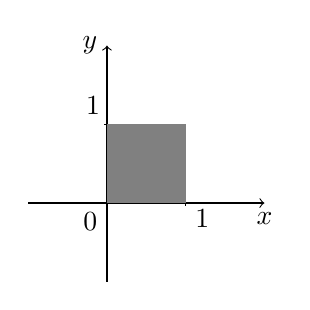
\begin{tikzpicture}
  \draw[->] (-1,0)--(2,0) node[below]{$x$};
  \draw[->] (0,-1)--(0,2) node[left]{$y$};
  \draw (-1pt,1)--(1pt,1) node[above left]{$1$};
  \draw (1,-1pt)--(1,1pt) node[below right]{$1$};
  \path (0,0) node[below left]{$0$};
  \fill[gray] (0,0) -- (1,0) -- (1,1) -- (0,1) -- cycle;
\end{tikzpicture}
